\documentclass[a4paper,11pt]{ctexbook}
\usepackage{mypreamble}
\begin{document}
\setcounter{chapter}{9}
\chapter{基本数据结构}
\section{栈和队列}
栈和队列都是动态集合,且在其上进行DELETE操作所移除的元素是预先设定的。在栈(stack)中,被删除的是最近插入的元素:栈实现的是一种\textbf{后进先出(last-in,first-out,LIFO)}策略。在队列(queue)中,被删去的总是在集合中存在时间最长的那个元素:队列实现的是一种\textbf{先进先出(first-in,first-out,FIFO)}策略。本节将介绍如何利用一个简单的数组实现这两种结构。

\textbf{栈}

如图10-1所示,可以用一个数组$ S[1 \cdots n] $来实现一个最多可容纳$ n $个元素的栈。该数组有一个属性$ S.top $,指向最新插入的元素。栈中包含的元素为$ S[1 \cdots S.top] $,其中$ S[1] $是栈底元素,而$ S[S.top] $是栈顶元素。
\begin{figure}[htbp]	
	\begin{center}
		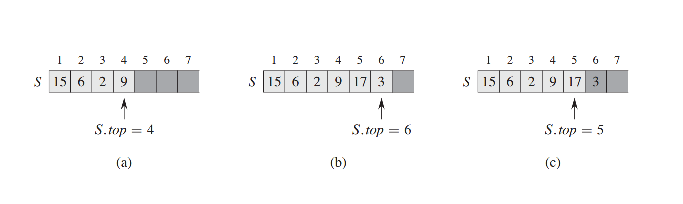
\includegraphics{figure/10.1.eps}	
		\caption{栈S的数组实现,只有出现在在浅灰色格子里的才是栈内元素。}
	\end{center}	
\end{figure}

当$ S.top = 0 $时,栈中不包含任何元素,即栈是空(empty)的。要测试一个栈是否为空可以用查询操作$ \proc{STACK-EMPTY} $。如果试图对一个空栈执行弹出操作,则称栈\textbf{下溢(underflow)},这通常是一个错误。如果$ S.top $超过了$ n $,则称栈\textbf{上溢(overflow)}。(在下面的伪代码实现中,我们不考虑栈的上溢问题。)

栈的几种操作只需分别用几行代码来实现:
\begin{codebox}
	\Procname{$ \proc{STACK-EMPTY}(S)$}
	\li \If $ \attrib{S}{top} \isequal 0 $
	\li \Then \Return TRUE
	\li \Else \Return FALSE	
\end{codebox}
\begin{codebox}
	\Procname{$ \proc{PUSH}(S,x)$}
	\li $ \attrib{S}{top} \gets \attrib{S}{top} + 1 $
	\li $ S[\attrib{S}{top}] \gets x $
\end{codebox}
\begin{codebox}
	\Procname{$ \proc{POP}(S) $}
	\li \If $ \proc{STACK-EMPTY}(S) $
	\li \Then error "underflow"
	\li \Else $ \attrib{S}{top} \gets \attrib{S}{top} - 1 $
	\li \Return $ S[\attrib{S}{top} + 1] $
\end{codebox}
上述三种操作执行的时间都为O(1)。

\textbf{队列}

队列上的INSERT操作称为入队(ENQUEUE),DELETE操作称为出队(DEQUEUE);正如栈的POP操作一样,DEQUEUE操作也没有参数。队列的先进先出特性类似于收银台前排队等待结账的一排顾客。队列有\textbf{队头(head)}和\textbf{队尾(tail)},当有一个元素入队时,它被放在队尾的位置,就像一个新到来的顾客排在队伍的末端一样。而出队的元素则总是排在队头的那个,就像排在队伍前面等待最久的那个顾客一样。
\begin{figure}[htbp]	
	\begin{center}
		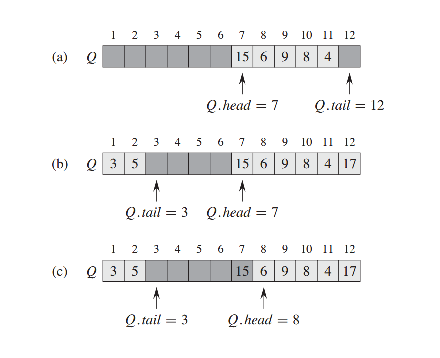
\includegraphics{figure/10.2.eps}	
		\caption{利用数组Q[1..12]实现一个队列。只有出现在浅灰色格子里的才是队列的元素。(a)队列包含5个元素,位于Q[7..11]。(b)依次调用ENQUEUE(Q,17)、ENQUEUE(Q,3)和ENQUEUE(Q,5)后队列的构成。(c)在调用DEQUEUE(Q)并返回原队头关键字15后,队列的构成。此时新的队头元素的关键字为6。}
	\end{center}	
\end{figure}

图10-2表面利用数组$ Q[1..n] $来实现一个最多容纳$ n-1 $个元素的队列的一种方式。该队列有一个属性$ Q.head $指向队头元素。而属性$ Q.tail $则指向下一个新元素将要插入的位置。队列中的元素存放在$ Q.head $,$ Q.head + 1 $,... ,$Q.tail-1$,并在最后的位置“环绕”,感觉好像位置1紧邻在位置n后面形成一个环序。当$ Q.head = Q.tail $时,队列为空。初始时有$ Q.head = Q.tail = 1 $。如果试图从空队列中删除一个元素,则队列发生下溢。当$ Q.head = Q.tail + 1 $时,队列是满的,此时若试图插入一个元素,则队列发生上溢。

在下面的ENQUEUE和DEQUEUE程序中,省略了对下溢和上溢的检查。在下列伪代码中,假设$ n = Q.length $。

\begin{codebox}
	\Procname{\proc{ENQUEUE}(Q,\id{x})}
	\li $ Q[\attrib{Q}{tail}] \gets x $
	\li \If $\attrib{Q}{tail} \isequal \attrib{Q}{length} $
	\li \Then $ \attrib{Q}{tail} \gets 1 $
	\li \Else $ \attrib{Q}{tail} \gets \attrib{Q}{tail} + 1 $
\end{codebox}
\begin{codebox}
	\Procname{\proc{DEQUEUE}(Q)}
	\li $ \id{x} \gets Q[\attrib{Q}{head}] $
	\li \If $\attrib{Q}{head} \gets \attrib{Q}{length}$
	\li \Then $ \attrib{Q}{head} \gets 1 $
	\li \Else $ \attrib{Q}{head} \gets \attrib{Q}{head} + 1 $
		\End
	\li \Return $ \id{x} $
\end{codebox}

图10-2 所示为 ENQUEUE 和 DEQUEUE 操作的执行结果。两种操作的执行时间都为O(1)

\section*{练习}
10.1-1 仿照图10-1,画图表示依次执行操作PUSH(S, 4)、PUSH(S, 1)、PUSH(S, 3)、POP(S)、PUSH(S, 8)和POP(S)每一步的结果,栈S初始为空,存储于数组S[1..6]中。

略

10.1-2 说明如何在一个数组A[1..n]中实现两个栈,使得当两个栈的元素个数之和不为 n 时,两者都不会发生上溢。要求PUSH和POP操作的运行时间为O(1)。


\end{document}
